\documentclass[]{elsarticle} %review=doublespace preprint=single 5p=2 column
%%% Begin My package additions %%%%%%%%%%%%%%%%%%%
\usepackage[hyphens]{url}

  \journal{The Journal of Mass Spectrometry:Applications to the Clinical
Laboratory} % Sets Journal name


\usepackage{lineno} % add
\providecommand{\tightlist}{%
  \setlength{\itemsep}{0pt}\setlength{\parskip}{0pt}}

\usepackage{graphicx}
\usepackage{booktabs} % book-quality tables
%%%%%%%%%%%%%%%% end my additions to header

\usepackage[T1]{fontenc}
\usepackage{lmodern}
\usepackage{amssymb,amsmath}
\usepackage{ifxetex,ifluatex}
\usepackage{fixltx2e} % provides \textsubscript
% use upquote if available, for straight quotes in verbatim environments
\IfFileExists{upquote.sty}{\usepackage{upquote}}{}
\ifnum 0\ifxetex 1\fi\ifluatex 1\fi=0 % if pdftex
  \usepackage[utf8]{inputenc}
\else % if luatex or xelatex
  \usepackage{fontspec}
  \ifxetex
    \usepackage{xltxtra,xunicode}
  \fi
  \defaultfontfeatures{Mapping=tex-text,Scale=MatchLowercase}
  \newcommand{\euro}{€}
\fi
% use microtype if available
\IfFileExists{microtype.sty}{\usepackage{microtype}}{}
\bibliographystyle{elsarticle-harv}
\ifxetex
  \usepackage[setpagesize=false, % page size defined by xetex
              unicode=false, % unicode breaks when used with xetex
              xetex]{hyperref}
\else
  \usepackage[unicode=true]{hyperref}
\fi
\hypersetup{breaklinks=true,
            bookmarks=true,
            pdfauthor={},
            pdftitle={Reproducible Manuscript Preparation with RMarkdown Application to JMASCL and other Elsevier Journals.},
            colorlinks=false,
            urlcolor=blue,
            linkcolor=magenta,
            pdfborder={0 0 0}}
\urlstyle{same}  % don't use monospace font for urls

\setcounter{secnumdepth}{5}
% Pandoc toggle for numbering sections (defaults to be off)

% Pandoc citation processing
\newlength{\csllabelwidth}
\setlength{\csllabelwidth}{3em}
\newlength{\cslhangindent}
\setlength{\cslhangindent}{1.5em}
% for Pandoc 2.8 to 2.10.1
\newenvironment{cslreferences}%
  {}%
  {\par}
% For Pandoc 2.11+
\newenvironment{CSLReferences}[3] % #1 hanging-ident, #2 entry spacing
 {% don't indent paragraphs
  \setlength{\parindent}{0pt}
  % turn on hanging indent if param 1 is 1
  \ifodd #1 \everypar{\setlength{\hangindent}{\cslhangindent}}\ignorespaces\fi
  % set entry spacing
  \ifnum #2 > 0
  \setlength{\parskip}{#2\baselineskip}
  \fi
 }%
 {}
\usepackage{calc} % for calculating minipage widths
\newcommand{\CSLBlock}[1]{#1\hfill\break}
\newcommand{\CSLLeftMargin}[1]{\parbox[t]{\csllabelwidth}{#1}}
\newcommand{\CSLRightInline}[1]{\parbox[t]{\linewidth - \csllabelwidth}{#1}}
\newcommand{\CSLIndent}[1]{\hspace{\cslhangindent}#1}

% Pandoc header
\usepackage{float}
\usepackage{booktabs}
\usepackage{longtable}
\usepackage{array}
\usepackage{multirow}
\usepackage{wrapfig}
\usepackage{float}
\usepackage{colortbl}
\usepackage{pdflscape}
\usepackage{tabu}
\usepackage{threeparttable}
\usepackage{threeparttablex}
\usepackage[normalem]{ulem}
\usepackage{makecell}
\usepackage{xcolor}



\begin{document}
\begin{frontmatter}

  \title{Reproducible Manuscript Preparation with RMarkdown
\newline \large Application to JMASCL and other Elsevier Journals.}
    \author[SPH,UBC]{Daniel T. Holmes\corref{1}}
   \ead{dtholmes@mail.ubc.ca} 
    \author[SPH,PHCDP]{Mahdi Mobini}
   \ead{mmobini@providencehealth.bc.ca} 
    \author[UO,TOH,EORLA]{Christopher R. McCudden}
   \ead{cmccudde@uottawa.ca} 
      \address[SPH]{St.~Paul's Hospital Department of Pathology and
Laboratory Medicine, 1081 Burrard St., Vancouver, BC V6Z 1Y6 Canada}
    \address[PHCDP]{Providence Health Digital Products, 1190 Hornby St.,
Vancouver, BC V6Z 2K5 Canada}
    \address[UBC]{University of British Columbia Department of Pathology
and Laboratory Medicine, 2211 Wesbrook Mall, Vancouver, BC V6T 1Z7
Canada}
    \address[TOH]{Department of Pathology and Laboratory Medicine,
Ottawa Hospital, General Campus, 501 Smyth Road, Ottawa, ON K1H 8L6
Canada}
    \address[UO]{Department of Pathology and Laboratory Medicine,
University of Ottawa}
    \address[EORLA]{Eastern Ontario Regional Laboratory Association}
      \cortext[1]{Corresponding Author}
  
  \begin{abstract}
  \textbf{Introduction}: With the rising complexity of modern
  multimarker analytical techniques and notable scientific publication
  retractions required for erroneous statistical analysis, there is
  increasing awareness of importance of research transparency and
  reproducibility. The development of mature open-source tools for
  literate programming in multiple langauge paradigms has made
  fully-reproducible authorship possible. \newline \textbf{Objectives}:
  We describe the procedure for manuscript preparation using RMarkdown
  and and the R stastical programming language with application to
  JMSACL or any other Elsevier journal. \newline \textbf{Methods}: An
  instructional manuscript is prepared in the RMarkdown markup language
  with stepwise directions on preparing sections, subsections, lists,
  tables, figures and reference management entirely reproducible
  format.\newline \textbf{Results}: From RMarkdown code, a
  submission-ready pdf is and JMSACL-compatible LaTeX code is generated.
  These can be uploaded to the Editorial Manager.\newline
  \textbf{Conclusion}: A completely reproducible manuscript preparation
  pipeline using the R and RMarkdown is described.\newline
  \end{abstract}
  
 \end{frontmatter}

\hypertarget{introduction}{%
\section{Introduction}\label{introduction}}

There is increasing attention paid to the concept of reproducible
research in the biological and medical sciences {[}1{]}. The problem of
poor reproducibility of biomedical research has been attributed to a
number of factors: study design, preanalytical handling, reagent lot
variation, suboptimal analytical reproducibility, researcher bias,
incorrect use of statistical methodologies, and unexpected artifacts of
software--even when working-as-designed.

Reproducibility in research has different components which have been
previously defined as i) methods reproducibility: protocols, measurement
procedures, reagents, data processing and analysis ii) results
reproducibility: the ability for an independent study to obtain similar
results in similar experimental conditions, iii) inferential
reproducibility: the ability of another researcher to draw the same
conclusions from the original data or a similar data set {[}2{]}.

One aspect of research reproducibility is statistical transparency which
primarily falls into the category of methods reproducibility but
encompasses some aspects of results and inferential reproducibility. A
concrete way to address statistical transparency is the so-called
``executable document'' or ``literate programming'' {[}3{]}. These terms
refer to a document that is itself a script or program that directly
pulls in the raw data for the study and reveals the entire statistical
methodology in the code. When the program or code is executed, it
produces a human readable document to which we are accustomed (e.g.~PDF,
Microsoft (MS) Word or HTML) complete with statistics and figures. The
use of reproducible research tools has become more common because of the
large and complex data sets on which modern clinical research is
performed and in response to conspicuous examples of serious inferential
error which would have been more easily detected (or perhaps avoided
entirely) were the research performed reproducibly to begin with
{[}4,5{]}.

While there are a number of approaches to reproducible document
preparation {[}6--8{]} perhaps the most mature of these is the use of
the R \textbf{knitr} package {[}9{]} and RMarkdown document format
{[}10{]} inside of the RStudio open-source development environment for
the R programming language.

In this article, we will review all aspects of reproducible manuscript
preparation for JMASCL using the R programming language and the
\textbf{rmarkdown} and \textbf{knitr} packages to generate all
calculated/rendered aspects of a manuscript including headers, sections,
figures, tables, captions, inline numerical results (including p-values
and confidence intervals), references, and reference formatting. The
result is LaTeX source code which can be submitted and/or compiled to
pdf. LaTeX (stylized as \LaTeX) is a versatile and powerful type setting
system used for publishing {[}11{]}.

\hypertarget{set-up}{%
\section{Set Up}\label{set-up}}

\hypertarget{necessary-software-installation}{%
\subsection{Necessary Software
Installation}\label{necessary-software-installation}}

The reader will need to install the R programming language on their
computer which is available for MacOS, Linux and Windows operating
systems {[}12{]}. Additionally, in order to generate LaTeX code from
which pdf files can be generated, it will be necessary to install the
LaTeX markup language, which can be installed in a dedicated manner
{[}11{]} or more simply by installing the R \textbf{tinytex} package
{[}13{]}. The reader should also install the RStudio integrated
development (IDE) environment {[}14{]}. In order to generate LaTeX
results immediately compatible with submissions to Elsevier journals,
the \textbf{rticles} {[}15{]} package is also required.

\hypertarget{creating-a-new-manuscript-template}{%
\subsection{Creating a New Manuscript
Template}\label{creating-a-new-manuscript-template}}

Once the necessary software is installed, from a new session in RStudio,
select File \textgreater{} New File \textgreater{} RMarkdown from the
menu and then when a window appears, select From Template and Elsevier
Journal Article as shown in figure 1. After entering the desired
filename and a directory into which you wish to save your manuscript,
click OK an the RMarkdown file template will appear. This template can
be modified as required and will compile when the ``Knit'' button is
selected, generating a PDF and the LaTeX source code which can be
submitted to JMSACL.

\begin{figure}[H]

{\centering 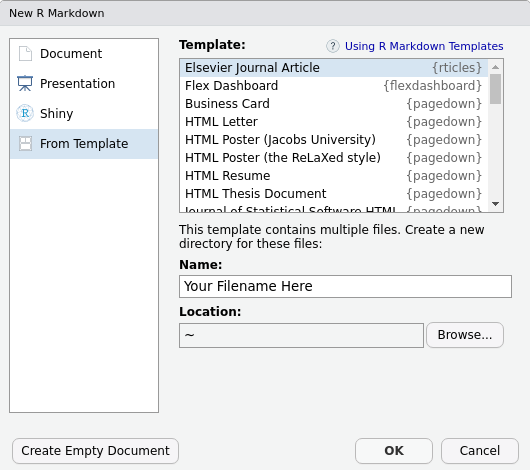
\includegraphics[width=0.6\linewidth,]{Figures/Figure1} 

}

\caption{RStudio selection window for Elsevier Journal Article}\label{fig:fig1}
\end{figure}

\hypertarget{proceeding-with-writing}{%
\section{Proceeding with Writing}\label{proceeding-with-writing}}

\hypertarget{title-page-and-front-matter}{%
\subsection{Title Page and Front
Matter}\label{title-page-and-front-matter}}

The LaTeX frontmatter of the article is generated by a YAML header at
the top of the document (YAML is a recursive acronym for ``YAML Ain't
Markup Language'' and serves as a human-readable configuration
language.) The content is contained between two sets of three dashes (-
- -), and being human-readable is fairly self-explanatory to modify. It
should be noted that it is \emph{very} sensitive to indentation and
spacing (unlike the R language) and care must be taken not to modify
either.

\hypertarget{markdown-basics}{%
\subsection{Markdown Basics}\label{markdown-basics}}

\hypertarget{sections-and-subsections}{%
\subsubsection{Sections and
Subsections}\label{sections-and-subsections}}

For sections of prose, RMarkdown uses the formatting of the Markdown
markup language, a complete review of which is not necessary as it is
extensively discussed elsewhere {[}16{]} (web resources and how-to tips
and syntax also are readily available,
e.g.~\url{https://rmarkdown.rstudio.com}). A named section of the
document is created with a \texttt{\#} followed by the section title,
subsections are made with \texttt{\#\#} and subsubsections with
\texttt{\#\#\#}. The code and corresponding document output is shown in
figure 2. It should be noted that carriage returns shown in the Markdown
code are required after the section name in order to generate the
desired output.

\hypertarget{italicization-and-bolding}{%
\subsubsection{Italicization and
Bolding}\label{italicization-and-bolding}}

Italicization of text is created by surrounding the text of interest
with single asterisks so that \texttt{*text\ written\ like\ this*} will
create output as \emph{text written like this}. Corresponding use of
double-asterisks will create bolded text so that
\texttt{**text\ written\ like\ this**} will create this bolded output:
\textbf{text written like this}.

\begin{figure}[H]

{\centering 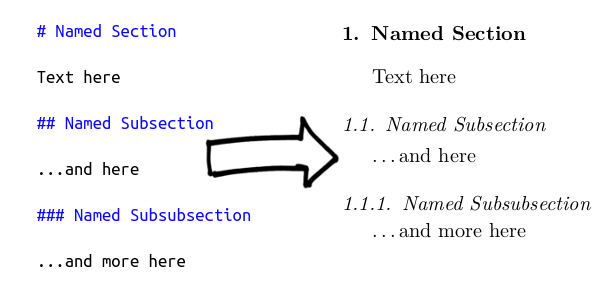
\includegraphics[width=0.75\linewidth,]{Figures/Figure2} 

}

\caption{How to define sections and subsections}\label{fig:fig2}
\end{figure}

A benefit of writing in plain text where everything is explicitly
encoded is that the author avoids the frustrations of hidden word
processor decisions about automatic correction, formatting of text,
bullets, and page breaks.

\hypertarget{bullets-and-numbered-lists}{%
\subsubsection{Bullets and Numbered
Lists}\label{bullets-and-numbered-lists}}

Bulleted lists are created with each item on a new line preceded by an
\texttt{*} while numbered lists are likewise created by a series of new
lines preceded by the corresponding number of the list. Indented
sublists are accomplished with indentation and the use of a \texttt{+}.

\begin{figure}[H]

{\centering 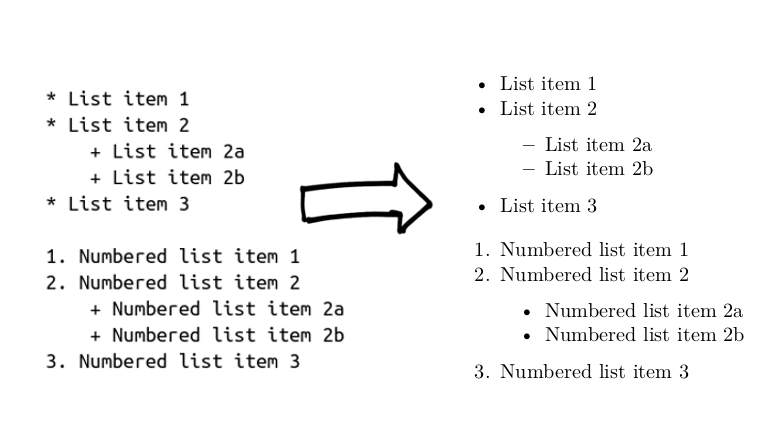
\includegraphics[width=0.9\linewidth,]{Figures/Figure3} 

}

\caption{Bulleted and numbered lists}\label{fig:fig3}
\end{figure}

\hypertarget{mathematics}{%
\subsubsection{Mathematics}\label{mathematics}}

RMarkdown allows the incorporation of beautifully rendered mathematics
using the syntax of LaTeX. Mathematics can typeset inline by surrounding
the mathematical expression by dollar signs so that
\texttt{\$\textbackslash{}Delta\ G\ =\ \textbackslash{}Delta\ G\^{}\{\textbackslash{}circ\}\ +\ RT\ \textbackslash{}ln\{Q\}\$}
will be rendered \(\Delta G = \Delta G^{\circ} + RT \ln{Q}\). If
mathematics is surrounded by \texttt{\$\$} on each side, it will be
typeset as a formula centered on a new line so that
\texttt{\$\$\textbackslash{}frac\{d\^{}2y\}\{dx\^{}2\}\ +\ (a-2q\textbackslash{}cos2x)y\ =\ 0\$\$}
is rendered:

\[\frac{d^2y}{dx^2} + (a-2q\cos2x)y = 0\]

\hypertarget{r-code}{%
\subsection{R Code}\label{r-code}}

The power of RMarkdown from the perspective of reproducible research is
the ability to embed R code chunks into the document so that the
statistical methodology is entirely exposed in the .Rmd file. The
readable output can be selected to show both the code and the output of
the code thereby making the whole analysis process both illustrative,
readable, and reproducible. Sections of code are created by the use of
code chunk delimiters
\texttt{\textasciigrave{}\textasciigrave{}\textasciigrave{}\{r\}} and
\texttt{\textasciigrave{}\textasciigrave{}\textasciigrave{}} like so:

\begin{verbatim}
```{r}
# generate 1000 random numbers: mean = 0 and sd = 1
z <- rnorm(1000,0,1)
# create a quick summary of the distribution
summary(z)
```
\end{verbatim}

The text appearing after the \# signs are explanatory comments which are
ignored by the R engine. The code above results in direct output from
the R console into the document:

\begin{verbatim}
##     Min.  1st Qu.   Median     Mean  3rd Qu.     Max. 
## -3.32078 -0.64970  0.03690  0.01681  0.70959  3.30415
\end{verbatim}

Generally it is undesirable to have R console (the code interface of R)
output print directly into a manuscript as shown above. For this reason,
all direct output of R's output, warnings, messages can all be
controlled with so-called chunk options. These options can be set
globally for the whole document or on a chunk-by-chunk basis as
required. For academic manuscripts, the following chunk option settings
suit most contexts:

\begin{verbatim}
```{r, echo = FALSE, warning = FALSE, message = FALSE}
# Chunk code here
```
\end{verbatim}

The above options suppress the R code in the document
(\texttt{echo\ =\ FALSE}), all R warnings (\texttt{warning\ =\ FALSE}),
and messages (\texttt{message\ =\ FALSE}), but permits variables to be
assigned and tables/figures to be generated. The following template used
can be used to set these globally:

\begin{verbatim}
```{r, include = FALSE}
knitr::opts_chunk$set(echo = FALSE, warning = FALSE, message = FALSE)
```
\end{verbatim}

\noindent The parameter \texttt{include=FALSE} permits code to run but
suppresses all console and graphical output.

All code chunk calculations are performed at the time of document
knitting by the R language interpreter and if the raw data input data
are updated, re-knitting will propagate all changes throughout the
document--including all figures, tables and inline text calculated from
R code. For an analyses with a large dataset, the re-rendering can take
time (picture re-running the entire analysis and figure rendering just
to change a typo), but can be managed by using `caches.' Caches save
parts of the analysis and are analogous to saving parts of webpages
enabling them to load faster. Parts that don't change, aren't
re-rendered. Like all things in R, caching of a chunk is optional and
controlled as follows:

\begin{verbatim}
```{r, cache = TRUE} 
# Computationally expensive code here
```
\end{verbatim}

It is customary (though optional) to name code chunks for the purposes
of quick identification and cross-referencing (through use of the
bookdown package described elsewhere {[}16{]}). Code chunk names must be
unique and are defined in the code chunk delimiter:

\begin{verbatim}
```{r, chunk_name} 
# Chunk code here
```
\end{verbatim}

\hypertarget{tables}{%
\subsubsection{Tables}\label{tables}}

For the purposes of illustration we will use a biomedical dataset
available in the \textbf{pROC} package taken from a 2010 study by Turck
et al examining blood biomarkers in patients suffering subarachnoid
hemmorhage {[}17{]}. The dataset has 7 variables named: 1. gos6: the
Glasgow Coma Outcome Score (1--6) 2. outcome: Clinical Outcome
(Good/Poor) 3. gender (M/F) 4. age 5. wfns: The World Federation of
Neurological Surgeons score (1--5) 6. s100b: S100 calcium-binding
protein B concentration (s100b in \(\mu\)g/L) and 7. ndka: Nucleoside
diphosphate kinase A concentration (nkda in \(\mu\)g/L).

While there are a number of ways to render a table into an RMarkdown
document, to our mind the simplest means is to prepare a dataframe of
results and to use the \texttt{kable()} function from the \textbf{knitr}
package {[}9{]} with the \textbf{kableExtra} package to permit many of
the complex table structures available natively in LaTeX {[}18{]}. With
these tools, a dataframe can be rendered as table easily as in the
following example code chunk.

\begin{center}\rule{0.5\linewidth}{0.5pt}\end{center}

\begin{verbatim}
```{r}
# call required libraries
library(pROC) 
library(kableExtra)
library(dplyr)
library(tidyr)
library(stringr)

# invoke the subarachnoid hemorrhage data set from the pROC package
data(aSAH) 

sah_frame <- aSAH %>%
  # group the cohort into Glasgow Coma Outcome Score 
  group_by(gos6) %>% 
  # produce summary statistics of age, s100b and NDKA
  summarise(
    median_age = median(age), 
    IQR_age = IQR(age),
    median_s100b = median(s100b),
    IQR_s100b = IQR(s100b),
    median_ndka = median(ndka),
    IQR_ndka = IQR(ndka)
  ) %>%
  # round all age columns to 1 decimal
  mutate(across(median_age:IQR_age,
                ~ sprintf(., fmt = '%.1f'))) %>%
  # round all biomarker columns to 2 decimals
  mutate(across(median_s100b:IQR_ndka,
                ~ sprintf(., fmt = '%.2f'))) %>%
  unite("Age", median_age:IQR_age, sep = " (") %>%
  mutate(Age = str_c(Age, ")")) %>%
  # bring biomarker results and their IQRs into one column
  unite("s100b", median_s100b:IQR_s100b, sep = " (") %>%
  mutate(s100b = str_c(s100b, ")")) %>%
  unite("ndka", median_ndka:IQR_ndka, sep = " (") %>%
  mutate(ndka = str_c(ndka, ")"))

caption <-
  "Summary table from the aSAH data set.\\
  Results are presented as median (IQR)"

# generate formatted output for table generation
sah_frame %>%
  kable(
    booktabs = "TRUE",
    format = "latex",
    align = 'cccc',
    col.names  = c("GOS6", "Age(y)", "S100b(ug/L)", "NDKA(ug/L)"),
    caption = caption
  ) %>%
  kable_styling(latex_options = c("HOLD_position", 'striped'), stripe_color = "#E0FAFA")
```
\end{verbatim}

\noindent The code chunk above first performs necessary calculations to
prepare a summary dataframe (a small table called a `tibble' more
precisely) and then renders table 1. Note that the formatting of all of
these outputs are infinitely customizable in terms of shading, row
highlighting, border styles, fonts, decimal places, and captions.

\begin{table}[H]

\caption{\label{tab:table1}Summary table from the aSAH data set.\
  Results are presented as median (IQR)}
\centering
\begin{tabular}[t]{cccc}
\toprule
GOS6 & Age(y) & S100b(ug/L) & NDKA(ug/L)\\
\midrule
\cellcolor[HTML]{E0FAFA}{1} & \cellcolor[HTML]{E0FAFA}{52.0 (21.2)} & \cellcolor[HTML]{E0FAFA}{0.29 (0.44)} & \cellcolor[HTML]{E0FAFA}{13.43 (9.81)}\\
3 & 57.0 (9.0) & 0.32 (0.42) & 13.56 (14.40)\\
\cellcolor[HTML]{E0FAFA}{4} & \cellcolor[HTML]{E0FAFA}{55.0 (16.0)} & \cellcolor[HTML]{E0FAFA}{0.12 (0.07)} & \cellcolor[HTML]{E0FAFA}{9.53 (6.80)}\\
5 & 49.0 (22.5) & 0.11 (0.09) & 10.95 (7.31)\\
\bottomrule
\end{tabular}
\end{table}

\hypertarget{figures}{%
\subsubsection{Figures}\label{figures}}

Figures generated by code chunks are inserted by default into the text.
Alternatively, they can be saved to a file to the image format required
by the journal. The following code chunk renders and inserts figure 4.
As an editorial side note for journal publishers, reviewers and authors
alike find no benefit in having tables and captions on separate pages
piled at the end of a manuscript.

\begin{center}\rule{0.5\linewidth}{0.5pt}\end{center}

\begin{verbatim}
```{r, fig.width = 5, fig.height = 4}
library(ggplot2)
library(cowplot)

# prepare a boxplot of s100b grouped by the World Federation 
# of Neurological Surgeons score
p1 <- aSAH %>%
  group_by(wfns) %>%
  ggplot(aes(x = wfns, y = s100b, fill=wfns)) +
  geom_boxplot() + 
  scale_fill_brewer(palette = "BuPu")+
  theme(legend.position = "none")  +
  ylab(expression('S100b (' * mu * 'g/L)'))+
  xlab("WFNS Classification")
  
# prepare a boxplot of NDKA grouped by the World Federation
# of Neurological Surgeons score  
p2 <- aSAH %>%
  group_by(ndka) %>%
  ggplot(aes(x = wfns, y = ndka,fill=wfns)) +
  ylim(c(0,100)) +
  geom_boxplot() +
  scale_fill_brewer(palette = "BuPu")+
  theme(legend.position = "none") +
  ylab(expression('NDKA (' * mu * 'g/L)'))+
  xlab("WFNS Classification")

# output the two plots side-by-side  
plot_grid(p1, p2, labels = "AUTO")
```
\end{verbatim}

\begin{figure}[H]
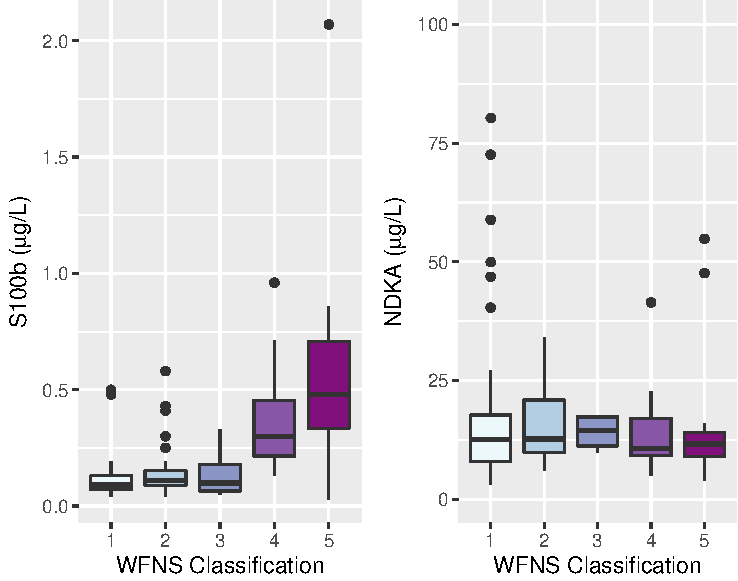
\includegraphics{JMSACL_Reproducible_files/figure-latex/fig4-1} \caption{Boxplots of s100b and NDKA concentrations as a function of world federation of neurological surgeons classification of SAH.}\label{fig:fig4}
\end{figure}

\hypertarget{inline-calculations}{%
\subsubsection{Inline calculations}\label{inline-calculations}}

It is frequently necessary to refer to results of a study within a
sentence. Under these circumstances, R code can be embedded inline
delimiting the code as follows:
\texttt{\textasciigrave{}r\ code\ goes\ here\textasciigrave{}}. For
example, this text:

\vspace{12pt}

\noindent The aSAH data set has
\texttt{\textasciigrave{}r\ nrow(aSAH)\textasciigrave{}} rows providing
biomarker results for
\texttt{\textasciigrave{}r\ table(aSAH\$gender){[}1{]}\textasciigrave{}}
males and
\texttt{\textasciigrave{}r\ table(aSAH\$gender){[}2{]}\textasciigrave{}}
females who suffered subarachnoid hemorrhage. The mean S100b for all
participants was
\texttt{\textasciigrave{}r\ round(mean(aSAH\$s100b),2)\textasciigrave{}}
\texttt{\$\textbackslash{}pm\$}
\texttt{\textasciigrave{}r\ round(sd(aSAH\$s100b),2)\textasciigrave{}}
\texttt{\$\textbackslash{}mu\$}g/L.

\vspace{12pt}

\noindent will result in this display which is calculated on the fly at
compilation:

\vspace{12pt}

\noindent The aSAH data set has 113 rows providing biomarker results for
42 males and 71 females who suffered subarachnoid hemorrhage. The mean
S100b for all participants was 0.25 \(\pm\) 0.27 \(\mu\)g/L.

This direct link between data analysis and manuscript preparation is
extremely powerful and likely to reduce errors by removing manual
transcription steps.

\hypertarget{reference-management}{%
\subsection{Reference Management}\label{reference-management}}

References are managed with LaTeX's reference management system,
BibLaTeX. The BibLaTeX references must be stored in a .bib text file
with entries in a prescribed syntax, which can be cut and paste from
Google Scholar, from the URL of the article itself or exported from
popular reference managers such as EndNote, Zotero and Mendeley. Jabref
is a notable cross-platform GUI reference manager dedicated to LaTeX.
The structure of .bib file entries is self-explanatory with most entries
appearing as follows:

\begin{verbatim}
@Article{Herold2016,
  title = {Building a foundation for clinical mass spectrometry
  and improved patient standard-of-care},
  journal = {Clinical Mass Spectrometry},
  volume = {1},
  pages = {1},
  year = {2016},
  issn = {2376-9998},
  doi = {https://doi.org/10.1016/j.clinms.2016.10.001},
  url = {https://www.sciencedirect.com/science/article/pii/S2376999816300289},
  author = {David Herold and Chris Herold}
}
\end{verbatim}

To cite the entry above one can simple write \texttt{@Herold2016} and
the numbered reference will appear in line {[}19{]} and in the
references section at the time of document knitting. Reference numbering
updates automatically each time the document is knit.

Formatting of references is dictated by the citation style language
(.csl) file referenced in the YAML header. The .csl file appropriate for
the journal of interest can be downloaded from the Zotero Style
Repository {[}20{]} and placed in the same folder as the .Rmd file. In
this case, the correct file is still referenced by the journal's prior
name, Clinical Mass Spectrometry.

\hypertarget{for-submission}{%
\subsection{For Submission}\label{for-submission}}

When an author is satisfied that their manuscript is ready for
submission to JMSACL, they may knit the document a final time. This will
generate a finalized LaTeX source file in the same folder as the .Rmd
file with the same name but with .tex file extension. There will also be
a folder generated also named according to the .Rmd file, in which there
will be a subfolder named figure-latex which contains all figures
generated from R code. Proceed with your submission via the Elsevier
Editorial Manager site submitting the pdf as your manuscript file and
the figures as per usual. Additionally, your .tex file, .bib file, and
.csl file must be submitted as a ``LaTeX Source File''

\hypertarget{discussion}{%
\section{Discussion}\label{discussion}}

We have outlined the process for preparing a manuscript reproducibly
using RMarkdown and RStudio. This process is suitable for any Elsevier
Journal and would only require minor modification for other journals.
Although many journals do not accept LaTeX as a submission format, it is
fairly easy to use the \textbf{bookdown} package {[}21{]} and to select
MS Word as the output format. As control of MS Word formatting is
somewhat more challenging from RMarkdown, some manual intervention may
be required after knitting depending on the author and journal
preferences.

We would be remiss not to underscore that the RMarkdown workflow permits
a fully transparent end-to-end data pipeline from the original data set
to the finished manuscript---a process we were not obliged to undertake
here because we are not working from any primary uncleansed data source.
However, all aspects of the data pipeline can be incorporated into R
code chunks, producing visible output as desired: the pre-processing
code (data cleansing), the analytical code (statistical analysis) and
the presentation code (tables and figures) {[}22{]}.

It is also important to note that within R code chunks one is able to
interact with databases (e.g.~SQL or Apache Spark) on the fly using
either native syntax or using R-code translated to SQL or Spark SQL by R
packages written for this purpose {[}23,24{]}. One can also insert code
from other languages such as Python {[}25{]} and Julia {[}26{]} as need
arises---for the convenience of not having to translate previously
developed source or to improve performance.

While a reader new to the concept of literate programming may not yet
perceive the need, preparation of a manuscript in RMarkdown permits the
use of a version-control system such as Git and a hosting system such as
\href{https://github.com/}{github}. These systems allow change-tracking,
collaboration and (when necessary) reversion to prior versions of the
source code. By this means not only the final product but all prior
incarnations are available for review. In contrast, traditional
GUI-based statistical and document preparation tools generally lack
mechanisms to track revisions. The RMarkdown source code for this
manuscript can be downloaded at
\href{https://github.com/drdanholmes/jmsacl_reproducible_research}{github.com/drdanholmes/jmsacl\_reproducible\_research}
{[}27{]}.

Notwithstanding the transparency that the RMarkdown workflow affords,
there still remains the problem that the R Language packages undergo
very rapid development, especially those associated with the popular
tidyverse suite {[}28{]}. This means that documents that properly knit
at present, may not knit in future because of package or function
modification and/or deprecation. However, solutions to this problem are
well-developed and the reader is encouraged to explore the use of the
renv and checkpoint packages. The \textbf{renv} package creates a local
R library within an R project {[}29{]}. Any R processes launched within
the project directory use the dedicated project library instead of the
user's regular R library, thereby guaranteeing future behaviour of the
code. Construction and reconstruction of local \emph{renv} libraries is
discussed in the appendix. The \textbf{checkpoint} and \textbf{packrat}
packages address the same problem with different strategies {[}30,31{]}.

Both of these package-dependency solutions may still have compatibility
problems, particularly as it pertains to the version of R itself. For
this reason perhaps the closest to being a definitive solution is
containerization with Docker or software container solution {[}32--34{]}
into which all necessary software is contained in a minimalistic image
that consumes much less resources than a virtual machine. The research
can then be shared as a Docker image without concern that any required
software is missing or out of date. For illustration purposes, we have
containerized this manuscript and its dependencies using Docker. The
Docker image is available at
\url{https://hub.docker.com/repository/docker/drdanholmes/jmsacl_reproducible_research}
and a description of how to use the image is provided in the appendix.

The readers should understand that writing a manuscript using literate
programming tools is more challenging and may be somewhat tedious in
comparison to using GUI wordprocessing and/or statistical programs.
Moreover, the process is probably slower {[}35{]}. Not all scientists
can or should be expected to become proficient in the use of Markdown,
R, or Python in order to be able to share their scientific findings.
Also challenging is the fact that reproducible research \emph{de facto}
requires the sharing of the raw data which scientists are reticent to do
since others might ``scoop'' them on new findings using their own data.
Additionally, data sharing introduces numerous questions and challenges
as it pertains to research ethics {[}36{]}.

Despite the comparative tedium of coding down to the sentence level, it
is important to note that manuscript changes required after expert
review are \emph{much easier} with a literate programming approach. If
incorporation of new data points is required, when the document is
re-knit, changes propagate automatically in inline code, tables and
figures provided content has not been hard-coded.

The use of GUIs for data analysis is often necessary in laboratory
medicine due to proprietary instrument file formats. However, laboratory
medicine and biomedical research communities have made many unforced
errors due to unwanted or unexpected behavior in the use MS Excel for
example {[}37{]} despite being prominently identified as problematic in
2004 {[}38{]}.

The availability and usability of notebook style tools report generation
tools for R and Python along with similar offerings for other languages
(e.g.~Julia, MATLAB, SAS and Stata) has made the bar much lower for the
biological and biomedical sciences to achieve transparent research
reproducibility. The onus is therefore on the publishers to push the
mandate of research reproducibility and on the universities and research
institutes to promote data science literacy to students. It bears
highlighting that these tools are also extremely valuable beyond peer
reviewed publishing. Literate programming offers complete documentation
and reproducibility in any clinical or research environment. It is
particularly useful for repetitive activities, such as method
evaluations, new lot validations, calibrations, and quality assurance.
The methods and templates can be built into standardized, parameterized
and transparent technical reports and template tools suited to a
particular lab or organization.

\hypertarget{conclusion}{%
\section{Conclusion}\label{conclusion}}

In summary, Rmarkdown offers a tremendous upside towards literature
programming and reproducible research. While it may initially seem odd
or intimidating, the tools are powerful, under the complete control of
the user, and entirely free. We hope that this article facilitates
students and researchers making the jump from ``mouse-moves'' to
programming and reproducible research.

\hypertarget{references}{%
\section*{References}\label{references}}
\addcontentsline{toc}{section}{References}

\hypertarget{refs}{}
\begin{CSLReferences}{0}{0}
\leavevmode\hypertarget{ref-munafo2017manifesto}{}%
\CSLLeftMargin{{[}1{]} }
\CSLRightInline{M.R. Munafò, B.A. Nosek, D.V. Bishop, K.S. Button, C.D.
Chambers, N.P. Du Sert, U. Simonsohn, E.-J. Wagenmakers, J.J. Ware, J.P.
Ioannidis, A manifesto for reproducible science, Nature Human Behaviour.
1 (2017) 1--9.}

\leavevmode\hypertarget{ref-goodman2016does}{}%
\CSLLeftMargin{{[}2{]} }
\CSLRightInline{S.N. Goodman, D. Fanelli, J.P. Ioannidis, What does
research reproducibility mean?, Science Translational Medicine. 8 (2016)
341ps12--341ps12.}

\leavevmode\hypertarget{ref-knuth_literate_1992}{}%
\CSLLeftMargin{{[}3{]} }
\CSLRightInline{D.E. Knuth, Literate {Programming}, 1st edition, Center
for the Study of Language; Inf, Stanford, Calif., 1992.}

\leavevmode\hypertarget{ref-baggerly2004reproducibility}{}%
\CSLLeftMargin{{[}4{]} }
\CSLRightInline{K.A. Baggerly, J.S. Morris, K.R. Coombes,
Reproducibility of SELDI-TOF protein patterns in serum: Comparing
datasets from different experiments, Bioinformatics. 20 (2004)
777--785.}

\leavevmode\hypertarget{ref-Baggerly2009}{}%
\CSLLeftMargin{{[}5{]} }
\CSLRightInline{K.A. Baggerly, K.R. Coombes, Deriving chemosensitivity
from cell lines: Forensic bioinformatics and reproducible research in
high-throughput biology, The Annals of Applied Statistics. 3 (2009)
1309--1334. \url{http://www.jstor.org/stable/27801549}.}

\leavevmode\hypertarget{ref-leisch2002sweave}{}%
\CSLLeftMargin{{[}6{]} }
\CSLRightInline{F. Leisch, Sweave: Dynamic generation of statistical
reports using literate data analysis, in: Compstat, Springer, 2002: pp.
575--580.}

\leavevmode\hypertarget{ref-poore2013reproducible}{}%
\CSLLeftMargin{{[}7{]} }
\CSLRightInline{G.M. Poore, Reproducible documents with pythontex, in:
Proceedings of the 12th Python in Science Conference, 2013: pp.
123--130.}

\leavevmode\hypertarget{ref-kluyver2016jupyter}{}%
\CSLLeftMargin{{[}8{]} }
\CSLRightInline{T. Kluyver, B. Ragan-Kelley, F. Pérez, B.E. Granger, M.
Bussonnier, J. Frederic, K. Kelley, J.B. Hamrick, J. Grout, S. Corlay,
others, {J}upyter {N}otebooks-a publishing format for reproducible
computational workflows., 2016.}

\leavevmode\hypertarget{ref-xie2018knitr}{}%
\CSLLeftMargin{{[}9{]} }
\CSLRightInline{Y. Xie, Knitr: A comprehensive tool for reproducible
research in {R}, in: Implementing Reproducible Research, Chapman;
Hall/CRC, 2018: pp. 3--31.}

\leavevmode\hypertarget{ref-allaire2021}{}%
\CSLLeftMargin{{[}10{]} }
\CSLRightInline{J. Allaire, Y. Xie, J. McPherson, J. Luraschi, K. Ushey,
A. Atkins, H. Wickham, J. Cheng, W. Chang, R. Iannone, Rmarkdown:
Dynamic documents for {R}, 2021.
\url{https://github.com/rstudio/rmarkdown}.}

\leavevmode\hypertarget{ref-latex_link}{}%
\CSLLeftMargin{{[}11{]} }
\CSLRightInline{{The LaTeX project}, (2021).
\url{https://www.latex-project.org/get/}.}

\leavevmode\hypertarget{ref-Rdownload}{}%
\CSLLeftMargin{{[}12{]} }
\CSLRightInline{{The Comprehensive R Archive Network}, (2021).
\url{https://cloud.r-project.org}.}

\leavevmode\hypertarget{ref-xie2019}{}%
\CSLLeftMargin{{[}13{]} }
\CSLRightInline{Y. Xie, TinyTeX: A lightweight, cross-platform, and
easy-to-maintain LaTeX distribution based on {TeX Live}, TUGboat. (2019)
30--32. \url{http://tug.org/TUGboat/Contents/contents40-1.html}.}

\leavevmode\hypertarget{ref-Rstudio}{}%
\CSLLeftMargin{{[}14{]} }
\CSLRightInline{RStudio Team, RStudio: Integrated development
environment for {R}, RStudio, PBC., Boston, MA, 2020.
\url{http://www.rstudio.com/}.}

\leavevmode\hypertarget{ref-rticles}{}%
\CSLLeftMargin{{[}15{]} }
\CSLRightInline{J. Allaire, Y. Xie, R Foundation, H. Wickham, Journal of
Statistical Software, R. Vaidyanathan, Association for Computing
Machinery, C. Boettiger, Elsevier, K. Broman, K. Mueller, B. Quast, R.
Pruim, B. Marwick, C. Wickham, O. Keyes, M. Yu, D. Emaasit, T. Onkelinx,
A. Gasparini, M.-A. Desautels, D. Leutnant, MDPI, Taylor and Francis, O.
Öğreden, D. Hance, D. Nüst, P. Uvesten, E. Campitelli, J. Muschelli, A.
Hayes, Z.N. Kamvar, N. Ross, R. Cannoodt, D. Luguern, D.M. Kaplan, S.
Kreutzer, S. Wang, J. Hesselberth, C. Dervieux, Rticles: Article formats
for r markdown, 2021. \url{https://CRAN.R-project.org/package=rticles}.}

\leavevmode\hypertarget{ref-rmarkdowndefinitive}{}%
\CSLLeftMargin{{[}16{]} }
\CSLRightInline{Y. Xie, J.J. Allaire, G. Grolemund, R markdown: The
definitive guide, Chapman; Hall/CRC, Boca Raton, Florida, 2018.
\url{https://bookdown.org/yihui/rmarkdown}.}

\leavevmode\hypertarget{ref-turck2010multiparameter}{}%
\CSLLeftMargin{{[}17{]} }
\CSLRightInline{N. Turck, L. Vutskits, P. Sanchez-Pena, X. Robin, A.
Hainard, M. Gex-Fabry, C. Fouda, H. Bassem, M. Mueller, F. Lisacek,
others, A multiparameter panel method for outcome prediction following
aneurysmal subarachnoid hemorrhage, Intensive Care Medicine. 36 (2010)
107--115.}

\leavevmode\hypertarget{ref-2021kableextra}{}%
\CSLLeftMargin{{[}18{]} }
\CSLRightInline{H. Zhu, kableExtra: Construct complex table with 'kable'
and pipe syntax, 2021.
\url{https://CRAN.R-project.org/package=kableExtra}.}

\leavevmode\hypertarget{ref-Herold2016}{}%
\CSLLeftMargin{{[}19{]} }
\CSLRightInline{D. Herold, C. Herold, Building a foundation for clinical
mass spectrometry and improved patient standard-of-care, Clinical Mass
Spectrometry. 1 (2016) 1.
https://doi.org/\url{https://doi.org/10.1016/j.clinms.2016.10.001}.}

\leavevmode\hypertarget{ref-Zoterostyles}{}%
\CSLLeftMargin{{[}20{]} }
\CSLRightInline{{Zotero Style Repository}, (2021).
\url{https://www.zotero.org/styles}.}

\leavevmode\hypertarget{ref-xie2021bookdown}{}%
\CSLLeftMargin{{[}21{]} }
\CSLRightInline{Y. Xie, Bookdown: Authoring books and technical
documents with {R} markdown, 2021.
\url{https://github.com/rstudio/bookdown}.}

\leavevmode\hypertarget{ref-peng2015report}{}%
\CSLLeftMargin{{[}22{]} }
\CSLRightInline{R. Peng, Report writing for data science in r, Lulu.
com, 2015.}

\leavevmode\hypertarget{ref-DBI}{}%
\CSLLeftMargin{{[}23{]} }
\CSLRightInline{R Special Interest Group on Databases (R-SIG-DB), H.
Wickham, K. Müller, DBI: R database interface, 2021.
\url{https://CRAN.R-project.org/package=DBI}.}

\leavevmode\hypertarget{ref-sparklyr}{}%
\CSLLeftMargin{{[}24{]} }
\CSLRightInline{J. Luraschi, K. Kuo, K. Ushey, J. Allaire, H. Falaki, L.
Wang, A. Zhang, Y. Li, The Apache Software Foundation, Sparklyr: R
interface to apache spark, 2021.
\url{https://CRAN.R-project.org/package=sparklyr}.}

\leavevmode\hypertarget{ref-Reticulate}{}%
\CSLLeftMargin{{[}25{]} }
\CSLRightInline{J. Allaire, K. Ushey, Y. Tang, D. Eddelbuettel,
Reticulate: R interface to python, 2017.
\url{https://github.com/rstudio/reticulate}.}

\leavevmode\hypertarget{ref-JuliaCall}{}%
\CSLLeftMargin{{[}26{]} }
\CSLRightInline{C. Li, {JuliaCall}: An {R} package for seamless
integration between {R} and {Julia}, The Journal of Open Source
Software. 4 (2019) 1284. \url{https://doi.org/10.21105/joss.01284}.}

\leavevmode\hypertarget{ref-drdanholmesgithub}{}%
\CSLLeftMargin{{[}27{]} }
\CSLRightInline{D.T. Holmes, 2021.
\url{https://github.com/drdanholmes/jmsacl_reproducible_research}.}

\leavevmode\hypertarget{ref-wickham2019}{}%
\CSLLeftMargin{{[}28{]} }
\CSLRightInline{H. Wickham, M. Averick, J. Bryan, W. Chang, L.D.
McGowan, R. François, G. Grolemund, A. Hayes, L. Henry, J. Hester, M.
Kuhn, T.L. Pedersen, E. Miller, S.M. Bache, K. Müller, J. Ooms, D.
Robinson, D.P. Seidel, V. Spinu, K. Takahashi, D. Vaughan, C. Wilke, K.
Woo, H. Yutani, Welcome to the {tidyverse}, Journal of Open Source
Software. 4 (2019) 1686. \url{https://doi.org/10.21105/joss.01686}.}

\leavevmode\hypertarget{ref-renv}{}%
\CSLLeftMargin{{[}29{]} }
\CSLRightInline{K. Ushey, Renv: Project environments, 2021.
\url{https://CRAN.R-project.org/package=renv}.}

\leavevmode\hypertarget{ref-ushley2021packrat}{}%
\CSLLeftMargin{{[}30{]} }
\CSLRightInline{K. Ushey, J. McPherson, J. Cheng, A. Atkins, J. Allaire,
Packrat: A dependency management system for projects and their r package
dependencies, 2021. \url{https://CRAN.R-project.org/package=packrat}.}

\leavevmode\hypertarget{ref-devries2020checkpoint}{}%
\CSLLeftMargin{{[}31{]} }
\CSLRightInline{A. de Vries, Microsoft, Checkpoint: Install packages
from snapshots on the checkpoint server for reproducibility, 2020.
\url{https://CRAN.R-project.org/package=checkpoint}.}

\leavevmode\hypertarget{ref-boettiger2015introduction}{}%
\CSLLeftMargin{{[}32{]} }
\CSLRightInline{C. Boettiger, An introduction to docker for reproducible
research, ACM SIGOPS Operating Systems Review. 49 (2015) 71--79.}

\leavevmode\hypertarget{ref-nust2019containerit}{}%
\CSLLeftMargin{{[}33{]} }
\CSLRightInline{D. Nüst, M. Hinz, Containerit: Generating dockerfiles
for reproducible research with r, Journal of Open Source Software. 4
(2019) 1603.}

\leavevmode\hypertarget{ref-chamberlain2014using}{}%
\CSLLeftMargin{{[}34{]} }
\CSLRightInline{R. Chamberlain, J. Schommer, Using docker to support
reproducible research, DOI: Https://Doi. Org/10.6084/M9. Figshare.
1101910 (2014) 44.}

\leavevmode\hypertarget{ref-knauff2014efficiency}{}%
\CSLLeftMargin{{[}35{]} }
\CSLRightInline{M. Knauff, J. Nejasmic, An efficiency comparison of
document preparation systems used in academic research and development,
PloS One. 9 (2014) e115069.}

\leavevmode\hypertarget{ref-meyer2018practical}{}%
\CSLLeftMargin{{[}36{]} }
\CSLRightInline{M.N. Meyer, Practical tips for ethical data sharing,
Advances in Methods and Practices in Psychological Science. 1 (2018)
131--144.}

\leavevmode\hypertarget{ref-ziemann2016gene}{}%
\CSLLeftMargin{{[}37{]} }
\CSLRightInline{M. Ziemann, Y. Eren, A. El-Osta, Gene name errors are
widespread in the scientific literature, Genome Biology. 17 (2016)
1--3.}

\leavevmode\hypertarget{ref-zeeberg2004mistaken}{}%
\CSLLeftMargin{{[}38{]} }
\CSLRightInline{B.R. Zeeberg, J. Riss, D.W. Kane, K.J. Bussey, E. Uchio,
W.M. Linehan, J.C. Barrett, J.N. Weinstein, Mistaken identifiers: Gene
name errors can be introduced inadvertently when using excel in
bioinformatics, BMC Bioinformatics. 5 (2004) 1--6.}

\leavevmode\hypertarget{ref-rprojects}{}%
\CSLLeftMargin{{[}39{]} }
\CSLRightInline{R. team, Using RStudio projects, 2021.
\url{https://support.rstudio.com/hc/en-us/articles/200526207-Using-Projects}.}

\end{CSLReferences}

\hypertarget{appendix}{%
\section*{Appendix}\label{appendix}}
\addcontentsline{toc}{section}{Appendix}

\hypertarget{using-the-renv-package-to-generate-a-local-library}{%
\subsection*{Using the renv package to generate a local
library}\label{using-the-renv-package-to-generate-a-local-library}}
\addcontentsline{toc}{subsection}{Using the renv package to generate a
local library}

The \emph{renv} package {[}29{]} permits the reconstruction of the R
library used at the time of authorship. In order to \emph{define} a
local library for others to use in future, one must define the RMarkdown
document as an R project {[}39{]} and execute the commands
\texttt{renv::init()} and \texttt{renv::snapshot()} within the project
context. This will generate a renv.lock file in the project folder which
defines the R and package repositories, package names, package versions,
and the hashes.

To \emph{reconstruct} the the library used to generate the RMarkdown
output of this manuscript, one must clone (or download) the
\href{https://github.com/drdanholmes/jmsacl_reproducible_research}{github
repository} {[}27{]} to their local machine, define it as an R project
(from an existing directory) as described in reference {[}39{]} and the
execute \texttt{renv::init()} and \texttt{renv::restore()}. This will
download all the correct versions of the R packages to a within-project
local library. When the RMarkdown file is knit, the local library will
be used.

If the version of R, pandoc or any other operating system dependencies
on the local machine differ from those used to generate the RMarkdown
output originally, warnings may result and there is finite that the
document will not compile. This can be overcome with the use of the
Docker.

\hypertarget{using-the-docker-container-to-generate-rmarkdown-output-reproducibly}{%
\subsection*{Using the Docker Container to Generate RMarkdown Output
Reproducibly}\label{using-the-docker-container-to-generate-rmarkdown-output-reproducibly}}
\addcontentsline{toc}{subsection}{Using the Docker Container to Generate
RMarkdown Output Reproducibly}

We have prepared a Docker container having all the Linux dependencies
and R package dependencies used for authorship of this manuscript. This
Docker file is optimized for this paper and may or may not work for
other RMarkdown files as it won't necessarily have all the required R
package dependencies.

To use our Docker container to generate the manuscript PDF, open a
command line shell session and navigate to a folder where you want the
PDF output to be produced. By executing the following commands you will:

\begin{enumerate}
\def\labelenumi{\arabic{enumi})}
\tightlist
\item
  pull the Docker image from the dockerhub repository
\item
  clone the manuscript github repository
\item
  navigate into the project folder
\item
  run the Docker image and issue a command to the Docker container to
  generate the PDF output.
\end{enumerate}

\begin{verbatim}
# Pulls the Docker image to your local machine's Docker engine
docker pull drdanholmes/jmsacl_reproducible_research

# Pulls down the gitub repository to the current working directory
git clone https://github.com/drdanholmes/jmsacl_reproducible_research.git

# Navigates to the downloaded project folder
cd jmsacl_reproducible_research

# Invokes the Docker container to process the .Rmd file to PDF
docker run --rm -it -w /home -v $PWD:/home m3d83/paper-jmsacl Rscript -e \
'rmarkdown::render("JMSACL_Reproducible.Rmd")'
\end{verbatim}

Should the user want to modify and rebuild the Docker image (to include
other R libraries for example), they may access the Dockerfile on the
\href{https://hub.docker.com/repository/docker/drdanholmes/jmsacl_reproducible_research}{Docker
Hub registry cited above} which is:
\url{https://hub.docker.com/repository/docker/drdanholmes/jmsacl_reproducible_research}


\end{document}

